\documentclass[10pt,letterpaper,twocolumn]{article}
% \usepackage{titlesec}
\usepackage[margin=0.8in]{geometry}
\usepackage[style=authoryear, backend=bibtex]{biblatex}
\pagenumbering{arabic}
\usepackage{lmodern}
\usepackage{graphicx}

% \usepackage{cogsci}
% \usepackage{pslatex}
\addbibresource{metaphor.bib}
\usepackage{mathtools}
\usepackage{parskip}
\usepackage{stmaryrd}
\usepackage{gb4e}
\usepackage{booktabs}
% \usepackage{hyperref}





\title{Bayesian Pragmatics with Distributional Semantics: a Computational Approach to Metaphor}
% \author{Reuben Cohn-Gordon and Leon Bergen \\ Stanford}
\date{}
% \titleformat*{\section}{\normalsize\bfseries}
\begin{document}
\maketitle



% \parskip
\begin{abstract}
\small
Previous Bayesian formalizations of the pragmatics of metaphor have required hand-crafted semantics and choices of utterance. We propose an elaboration of \citep{kao} which rests on a word embedding semantics, thereby replacing hand-crafted knowledge with information encoded in pretrained word vectors. We show that this model can interpret metaphors of the form ``A is a B'', by identifying the properties of B that are relevant to A. This work forms part of a more general project of scaling Bayesian models of pragmatics to real world data and distributional semantics.
\end{abstract}

% to add: jokes: he was as tall as a 6 foot three inch tree

% 		SEE NLU notebook for all of these
	% success of pretrained word embeddings: turney2010frequency
	% semantically close words are close in vector space: turney2010frequency
	% word vectors used in computational semantics: 
	% bayesian prob: citation: frank2012predicting
	% compositional distributional semantics: socher2013recursive
	% chomsky: infinite utterances: chomsky2002syntactic
	% linguists on metaphor: lakoff2008metaphors
	% cogscis on met
	% experimental work in RSA: basic stuff: frank?



Metaphor presents a compelling theoretical challenge for semantics and pragmatics, with corresponding tasks for NLP, of metaphor identification, understanding and paraphrase. As such, it has proven to be a topic of interest among philosophers (\cite{black}, \cite{davidson}) and linguists (\cite{lakoff2008metaphors}), and recently has seen much work in computational modeling (\cite{shutova2016design}). 


Pragmatic accounts of metaphor, stemming from (\cite{davidson}) and (\cite{grice}), attempt to derive metaphorical meaning as the inference of a language user reasoning about an expression heard in a given context. Grice suggests that a listener infers that a heard expression is metaphorical on account of the unlikelihood of its literal interpretation being true.
% 	fix this: should be: example of key importance:
% As \cite{shutova} notes, core NLP tasks such as translation often require an understanding of metaphor:
% 		The train of progress stormed across the country

			% examples only apply if metaphor is conventionalized: otherwise you could just translate the metaphor:

				% possibly not always: John is a shark

% Accounts of metaphor can be broadly divided on the basis of whether they treat metaphor as a semantic or pragmatic phenomenon. The former camp (e.g. \cite{lakoff}), treats metaphor as a fundamental part of semantic meaning, or even thought. The latter,


Within the paradigm of Bayesian pragmatics\footnote{See \cite{frank2012predicting} for an introduction to the Rational Speech Acts (RSA) model more generally} (\cite{kao}) proposes a model which conducts joint inference over the attributes of a referent and a \emph{question under discussion}. This Bayesian formalization offers not only a way to recognize that metaphorical expressions are not to be interpreted literally, like Grice suggests, but also a way to access the meaning the metaphor \emph{does} convey.

		

This Bayesian model offers a natural formalization of the intuitions of earlier pragmaticists and has allowed for rigorous experimental investigation. A further use of RSA in is computational models of semantics and pragmatics; recent work (e.g. \cite{andreas}, \cite{monroe2015learning}) has focused on integrating these Bayesian models with modern advances in computational linguistics.

Our contribution to this enterprise focuses on incorporating word vector semantics into RSA. To this end, we implement a model of RSA which has an infinite number of world states, which correspond to points in a word vector space. Furthermore, we implement a more complex variant of RSA (based on the work of \cite{kao}) that involves a notion of QUDs, so that the model reasons about which \emph{aspects} of word meaning are relevant to a given metaphor.

		% , showing that

		% 	computationally 
		% 		blah
		% 			implementations of RSA can model more that scalar implicature
		% 				chris will obviously tear this apart




% Given the success of word embeddings at a range of linguistic tasks (see \cite{turney2010frequency}), it is natural to wonder whether such embedding spaces can provide a knowledge base for a model of metaphor which is scalable to real world data.

% Building on the work of (\cite{kao}), we design and implement a distributional Bayesian model of metaphor meaning, which applies RSA to a semantics grounded in pretrained word embeddings. 

This model, which we refer to as DistRSA, allows us to generalize the RSA model of metaphor well beyond the hand-constructed examples which previous pragmatic models require. We apply our model to two task, which we view as crucial to the computational processing of metaphorical language: metaphor understanding, and metaphor detection.


	% The goal of a speaker is to produce an utterance which informs their interlocutor of the speaker's position in this space, to which end they may employ metaphorical language. For instance, if John is a ruthless businessman, then the sentence ``John is a shark.'' should enable the listener to infer John's position in the space.



We focus on predicative metaphors of the form ``A is a B'' (e.g. ``John is a shark.''), as well as metaphorical modification, e.g ``fiery temper'' or ``golden opportunity''. We further consider the possibility that the meaning of metaphorical phrases such as these can be interpreted as the posterior position of the head noun, after the model observes the modifying adjective.

We begin with a brief introduction to the RSA paradigm. We then sketch out how RSA, in particular QUD RSA can be applied to a distributional model of semantics, and describe the technical challenges this involves.

\section{Defining Metaphor}

% From a certain perspective, anything and everything is metaphorical. While we are theoretically sympathetic to a perspective in which metaphorical and literal meaning exist on a continuum, it is helpful to be clear about the sorts of cases we are interested in.

Metaphor exists in many syntactic forms, and generally eludes easy definition. For present purposes, we focus on metaphorical \emph{predication}, and in particular, copular predication of the form: ``A is a B''. These are cases where a predicate only applies to an entity in certain regards. What these regards are is contextually determined. Thus, \emph{being a rock} conveys different things for each of the following:

	\begin{exe}
	\ex
	% \item ``The garden fence is a brick wall'': with respect to being a brick wall.
	 ``That piece of granite is a rock.'' 
	 % : literal.
	 \label{first}
	\ex
	 ``That bread is a rock''
	 % : with respect to being hard. (Paraphrase: ``The bread is stale.'')

	\ex

	%  ``The bouncer at the nightclub is a brick wall'': with respect to being unyielding.
	 ``That unconscious man is a rock.'' 
	 % : with respect to being unchanging. (Paraphrase: ``The patient is unresponsive.'')

	\label{third}
	\end{exe}

The first example above is one of literal predication: the granite really is a rock. For the other two cases, however, only certain aspects of rocks are shared between subject and predicate. For example, the bread shares the property of hardness with a rock, while the unconscious man shares the property of unresponsiveness. The task of metaphor understanding can be summed up as the identification of which properties of the predicate are relevant to a given metaphor.

Parallel to metaphorical predication, one also finds cases of modification where an adjective modifies a noun in certain regards and not others. Thus, a \emph{fiery temper} shares with fire different properties to a \emph{fiery dish}, and in turn, both differs from a more literal usage, as with a \emph{fiery stove}.

A key property of metaphor is its productivity: it is not possible to enumerate every metaphorical sentence or phrase and its meaning. However, it should be noted that metaphors very commonly conventionalize into idiomatic phrases, to the point that predicates used metaphorically often absorb the metaphorical meaning into their literal meaning. Thus, ``John is a fool.'' would rarely, at present, be interpreted to mean that John performs dances and songs in a monarch's court. One the other hand, ``John is a butcher.'' could either mean that he processes meat (literal), or that he is violent (metaphorical), depending on the context.

While metaphors \emph{can} conventionalize into idioms, it not would be possible for a computer to understand metaphor simply by rote memorization of phrasal meanings; the semantic productivity of metaphor prevents this. This aside, the problem remains of using context to establish when an utterance or phrase is literal and when it is metaphorical. It is this productivity and contextuality which, in our opinion, merits the use of a probabilistic generative model. 

% anything which has an implicit meaning which can't be rooted in the conventional meaning: test: with respect to

% We offer two forms of evaluation, with and without human supervision, to demonstrate the success of the model

% Finally, we conclude with some remarks on the distinction between literal and metaphorical meaning which our model sheds light on
\section{Distributional Semantics} \label{distmods}

Distributional models of word meaning have proven hugely useful in a variety of applications in computational linguistics and NLP. These assign each word in a language a point in a high-dimensional vector space. It is possible to learn mappings from words to points roughly according to co-occurrence between neighboring words observed in large text corpora, so that words which appear in similar contexts are close in the vector space under cosine distance. Such word vectors can then encode both linguistic information (e.g. the similarity of verbs in the past tense) and world knowledge, e.g. the similarity of cats and dogs (see \cite{finley2017analogies}).


Google's Word2Vec (\cite{mikolov2013distributed}) and Stanford's GloVe (\cite{pennington2014glove}) are two standard models used to produce such vectors. Sets of word vectors produced by both models applied to very large amounts of text are publicly available.

Pretrained word embeddings appear to encode syntactic and semantic information (\cite{mikolov2013linguistic}), and as such, are useful element in many NLP tasks such as sentiment analysis (\cite{socher2013recursive}).

% are commonly used in NLP tasks that involve semantic information, such as sentiment analysis (\cite{}) and natural language entailment (\cite{bowman}).
% 	deep learning one
% 	abstractness
% 	sentiment analysis
	
	% (\cite{pennington2014glove}) argues that GloVe vectors exhibit a degree of linear structure, in the sense that for various quadruples of words (A,B,C,D), such that A is to B as C is to D, the corresponding pretrained vectors approximately satisfy the equation $\overrightarrow{\text{A}} - \overrightarrow{\text{B}} = \overrightarrow{\text{C}} - \overrightarrow{\text{D}}$, where $\overrightarrow{\text{A}}$ is the word vector corresponding to the word A. For instance, the nearest word vector by cosine distance to the point ($\overrightarrow{\text{king}}-\overrightarrow{\text{man}}+\overrightarrow{\text{woman}}$) in the Word2Vec embedding space is $\overrightarrow{\text{queen}}$.
	
	% % A shared property of both GloVe and Word2Vec is an approximately 


	% Pretrained word embeddings are used in deep learning systems as a form of transfer learning: for example, language models for translation and other tasks are greatly helped by representing words with pretrained GloVe or Word2Vec vectors, rather than learning them from scratch.


	Because of the rich semantic information encoded in word embeddings, many attempts have been made to utilize them for computational tasks requiring semantic understanding, such as sentiment analysis (\cite{socher2013recursive}) and abstractness detection (\cite{turney}).

% These usages of word vectors often blur the word/object distinction, in the sense that the pretrained embeddings can be understood to provide \emph{world} knowledge rather than solely knowledge about language. Thus, the vector associated with the word ``cat'' can be interpreted as its denotation, giving information about the animal \emph{cat}.

Metaphor is an obvious candidate for approaches that use distributional semantics: a wide variety of attempts have been made to leverage the information inherent in pretrained word vectors for the detection, interpretation and paraphrase of metaphor (see \cite{shutova2016design} for a comprehensive overview of proposed systems.).

An intuition which is voiced in many of these approaches is that metaphorical predicates should agree with only certain features of the subject. For instance:
\begin{quote}	``Computing a meaning always involves activating context-appropriate features and inhibiting or deactivating inappropriate features.'' (\cite{kintsch})
\end{quote}

A similar point is made about adjective-noun (AN) composition by (\cite{grefenstette2013category}): \begin{quote} ``In turn, through composition with its argument, I expect the function for such an adjective to \emph{strengthen} the properties that characterise it in the representation of the object it takes as argument.''
\end{quote}

Here, Grefenstette is suggesting that an adjective A, when modifying a noun N, targets certain properties of N and not others. He exemplifies this point as follows: ``When I apply ``angry'' to ``dog'' the vector for the compound ``angry dog'' should contain some of the information found in the vector for ``dog''. But this vector should also have higher values for the basis weights of ``fighting'', ``aggressive'' and ``mean'', and correspondingly lower values for the basis weights of ``passive'', ``peaceful'', ``loves''.''

In the philosophical literature on metaphor, a more abstract version on this idea that only certain aspects matter is alluded to by (\cite{black}), where for a metaphor ``A is a B'', Black refers to ``A'' as the ``principal subject'' and ``B'' as the ``subsidiary subject'':
		\begin{quote}
``We can say that the principal subject is  ``seen through'' the metaphorical expression - or, if we prefer, that the principal subject is ``projected upon'' the field of the subsidiary subject.'' - (\cite{black})
\end{quote}

Black offers the example of the metaphorical description of a war as a game of chess, commenting that ``the chess vocabulary filters and transforms: it not only selects, it brings forward aspects of the battle that might not be seen at all through another medium''.

The Bayesian model of metaphor proposed by (\cite{kao}) offers a way of capturing this dynamic of caring about certain aspects of the subject and not others: in this model, a listener jointly infers a Question Under Discussion (QUD), which dictates which aspects of the modifier or predicate to care about, and a world state, based on the information about the subject. This sort of joint inference of world state and topic or QUD is absent from previous distributional approaches to metaphor.

Our proposal is to unite distributional semantics with Bayesian pragmatics by constructing an RSA model of metaphor which uses word vectors. In this setting, world states will become vectors in the space and QUDs will be orthogonal projections which map these vectors to vectors in subspaces of the space.

We now review the general RSA framework, as well as the non-literal extension to RSA (\cite{kao}) on which our model will build.
	% The work closest to this, to our knowledge, is \cite{kintsch}, which proposes a single scheme for literal and metaphorical predication.

% However, we believe that in order to succeed fully at tasks involving metaphor, it is necessary to explicitly model a joint inference over QUDs and world states.


% \subsection{Intermixing of Word and Object}

% % In distributional RSA, both the world state and the utterance are represented as points in the same vector space as each other. This may appear strange to a semanticist: the denotations of words should not, intuitively, occupy the same type as that of possible worlds.

% What sort of knowledge dist models represent: word or object

% 	best here thought of as models of latter
% 	we'll treat them as giving a semantics, rather than being a mere cooccurence space

% 	The distributional setting in which our model exists requires a blurring of the line between knowledge of language and knowledge of the world. To put it another way, it might first seem odd that in our model, a speaker's knowledge of what a particular lawyer is like exists in the same space as their knowledge of the \emph{meaning} of the word \emph{shark}.



% 	Thus, for the purposes of our model, it is useful to think of a word vector space as a semantic space

\section{An Introduction to RSA} \label{rsa}

Bayesian probability provides an elegant and practical way of formalizing pragmatics (\cite{frank2012predicting}). For a comprehensive and basic introduction, we recommend \url{http://gscontras.github.io/ESSLLI-2016/chapters/1-introduction.html}.

The general form of the model posits listeners and speakers, both of which are represented as conditional probability distributions. Speakers are of the form $P(U\vert W)$ while listeners are $P(W\vert U)$, where $W$ is the type of the world and $U$ is the type of utterances. Thus, speakers are distributions over possible utterances given worlds, and listeners are distributions over possible worlds given utterances.

RSA works by defining successive levels of speaker and listener recursively. $L_0$, the most basic listener, conditions on the truth of an utterance u in order to update their prior on worlds. For this, we need a semantics, in the form of an interpretation function I of type ($U$,$W$ $\to \{0,1\}$).Formally, where $P(w)$ is the prior on worlds, and I is an interpretation function:

% \footnote{This semantics can be generalized to `soft RSA'', where the result type of I is the real interval from 0 to 1.}. 
\begin{exe}
\ex  $L_0(w\vert u) \propto  I(u,w)*P(w)$ \label{l0def}
\end{exe}


For instance, consider a game in which a speaker is shown a picture of either a shark or a goldfish, and must try to communicate which picture they see to a listener who hasn't seen the picture. Further suppose that the speaker is only allowed to make one of the single word utterances \emph{wet} or \emph{vicious}.

Supposing that it is true that both sharks and goldfish are wet, but that only sharks are vicious, one might imagine that on hearing \emph{wet}, a listener reasons as follows: if the speaker had wanted to convey that the picture was of a shark, they would have said \emph{vicious}, since this would be the least ambiguous thing to say in this situation. Since they didn't say \emph{vicious}, the picture is most likely of a goldfish.

We can formalize this reasoning process as follows in RSA. Here, the set of worlds $W$ is \{shark,goldfish\}, and the set of utterances $U$ is \{\emph{wet},\emph{vicious}\}\footnote{In this example (and in DistRSA), $U$ is finite. This is a modeling assumption, since linguistic agents do not really have a finite set of utterances (see \cite{chomsky2002syntactic}).}. We then define a semantics $\mathcal{I}$:

\begin{itemize}
\item $\mathcal{I}(\mathit{shark},\mathit{wet}) = 1$
\item $\mathcal{I}(\mathit{shark},\mathit{vicious}) = 1$
\item $\mathcal{I}(\mathit{fish},\mathit{wet}) = 1$
\item $\mathcal{I}(\mathit{fish},\mathit{vicious}) = 0$
\end{itemize}

We can now model a literal listener, $L_0$, who on hearing an adjective uttered tries to deduce which animal, a shark or a goldfish, is being referred to. $P(w)$ is here taken to be a uniform distribution, which encodes the assumption that before hearing anything, $L_0$ thinks either picture is equally likely to be referred to.

\begin{exe}
\ex $L_0(w\vert u)) \propto \mathcal{I}(w,u) * P(w)$ \label{simplelzero}
\end{exe}


$S_1$ chooses their utterance in order to best convey which world they are in (that is, which image they have been presented with). We define $S_1$'s utility function in (\ref{utilityfunc}) and $S_1$ in (\ref{s1simplersa}):



\begin{exe}
\ex $U(u,w) = \log(L_0(w\vert u))$ \label{utilityfunc}
\ex $S_1(u\vert w) \propto e^{U(u,w)}$ \label{s1simplersa}
\end{exe}

Note that $S_1$ is more likely to say \emph{vicious} when presented with \emph{shark} than \emph{wet}. $L_1$, in turn, conditions on $S_1$ being in a world which would have produced the heard utterance:
\begin{exe}
\ex $L_1(w\vert u) \propto S_1(u\vert w)*P(w)$
\end{exe}

$L_1$, on hearing \emph{wet}, will place more mass on \emph{fish} than \emph{shark}, which models the reasoning process described above.

		% This means that if the $L_1$ will update their prior so that the most likely world is the one corresponding to the exact height the received utterance denotes. So if the $L_1$ hears that Tarksi is 6 feet tall, they will infer that he is no more than 6 feet tall, since, if he had been, the informative $S_1$ would have said an utterance denoting a greater height. This inference corresponds to the notion of \emph{scalar implicature} - when speaking to an $L_1$ listener, it is possible to \emph{imply} that Tarski is exactly 6 feet tall by saying that he is at least 6 feet tall. Therefore the information conveyed is greater than the strict literal meaning of the utterance. 


		% For instance, suppose worlds are simply values corresponding to the height of some person, say, Alfred Tarski, and that utterances denote his height too. On hearing the utterance ``6 feet'', the literal listener will update his prior on possible worlds so that it only includes worlds in which Tarski is at least 6 feet tall.

		% The speaker, $S_1$ attempts, in turn, to produce the utterance u which maximizes a utility function U. For the simplest case of RSA, we define U as

		% % \footnote{Basic enrichments to this setup include the subtraction of a cost term from U(u$\vert$w), and a so-called ``rationality parameter'' which multiplies U(u$\vert$w).}:


		% Using the utility function in (\ref{utility}) and assuming a uniform prior on utterances, we obtain a distribution for $S_1$ proportional to the utility:
		% \begin{exe}
		% \end{exe}

		% Informally, this means that the speaker will most favor the utterance which denotes the exact height that the speaker believes Tarski to be. Any utterance denoting a lesser height will be true in our semantics and therefore will have some utility, but will be strictly less informative than saying the exact height. Importantly, utterances denoting a greater height receive no utility and are ruled out, since they would lead the $L_0$ to a world incompatible with the speaker's world. This means that it is necessary to add something to the model in order to deal with non-literal utterances (i.e. utterances which are false relative to the speaker's world).


RSA requires hand-constructed inputs for three aspects of the model: the semantics used in $L_0$, the set of possible utterances in $S_1$, and the set of world states in $L_0$ and $L_1$.

% In our current example, the semantics is a mapping f the meaning of an utterance is a real number, and the possible utterances are a set of real numbers. Even here, however, it is necessary to choose some discrete set of real numbers which are valid utterances, by hand.

These three hand-constructed inputs are controlling factors on the scalability and domain-genericity of RSA, since each case of RSA requires the provision of all three. As we shall see, RSA with Questions under Discussion introduces a fourth such controlling factor: the need for a predetermined set of QUDs to be provided to the model.

\section{RSA with QUDs} \label{rsawithqud}



	% On hearing ``John is a shark.'', a listener, whose prior on John literally being a shark is very low, infers that the speaker is talking metaphorically.

	% While this account explains how a listener might infer that (\ref{}) is not meant literally, it has very little to say about what metaphor \emph{does} mean.



(\cite{kao}) proposes a model of metaphors of the form ``A is a B'' in which world states are a set of Boolean properties of A. Accordingly, a listener's prior belief is their knowledge about what A is like before hearing ``B''. The model must then account for how a listener is able to hear ``A is a B'', and only update their beliefs about A with regards to certain properties of B. For instance, on hearing that the lawyer is a shark, I may conclude that the lawyer is bloodthirsty, but not that she has gray skin.  

To account for this, (\cite{kao}) introduces an additional feature to RSA. This is the notion of a Question under Discussion, inspired by the related notion of the same name proposed by (\cite{roberts1996information}).
% in order to model non-literal meaning such as metaphor and hyperbole in empirically plausible ways (see \cite{kao} for experimental verification of this claim). 

In the context of RSA, a QUD can be understood as a function of type (W$\to$powerset(W)), which discards certain information about the world. For instance, suppose we have a model in which worlds consist of triples of properties pertaining to a subject, e.g. the lawyer in the sentence ``The lawyer is a shark.''. One such world might look like: $\langle$c(lever)=True,v(icious)=True,a(quatic)=False$\rangle$. 

Denotations of utterances, like \emph{shark} in the above example, are distributions over world states. As before, we  define a function $\mathcal{I}$, which here takes a word x and a world y, and returns the probability density of y in the denotation of x. This allows us to define an $L_0$ model identical to that of standard RSA (see (\ref{simplelzero})):

\begin{exe}
\ex  $L_0(w\vert u) \propto  \mathcal{I}(u,w)*P(w)$
\end{exe}

Here, $P(w)$ is the listener's prior over worlds, which encodes the information known about the subject of the metaphor (e.g. the lawyer) before hearing ``shark''. For instance, let us suppose that worlds in which \emph{aquatic} is true of the laywer have little probability mass in this prior distribution. This represents our prior knowledge that lawyers cannot breathe underwater. This $L_0$ is much like the standard RSA $L_0$ defined in (\ref{simplelzero}).

% The $L_1$ will have the same prior on worlds.

% In this setting, 

% As for the $L_0$ prior distribution, let us suppose it is a distribution over world triples, such 

% We could imagine a distribution which is not uniform, and puts more weight on worlds in which lawyers are clever.

The first key difference to simple RSA comes at the $S_1$, which takes both a world and QUD. In this setting, a QUD is a function which maps any world triple to some element of that triple\footnote{Or equivalently, to the set of worlds which agree on that element.}. For example, the QUD which maps worlds to their first argument would be the \emph{cleverness} QUD, the QUD that only cares about whether the lawyer is clever.

% , and chooses an utterance according to how well it communicates the \emph{aspect} of the world that the QUD cares about.

The $S_1$, of type P(w$\vert$u,q), for an utterance u and QUD q, chooses the utterance which causes the listener's world state after hearing u to be the same as the speaker's world state \emph{under the QUD}. Formally:

\begin{exe}
\ex U(u,w,q) = $\log(\sum_{w'} \delta_{q(w)=q(w')} * L_0(w'\vert u))$
\ex $S_1(u\vert w,q) \propto e^{U(u,w,q)}$
\end{exe}


% \footnote{Note that in such a scenario, our world state is the state of the lawyer, as regards certain attributes.} 

% (\cite{kao}) has world states of exactly this sort. 

% For (\cite{kao}), utterances are nouns describing the subject, such as ``shark'', ``human'', etc. 

% Formally, the $L_0$ is identical the the simple RSA $L_0$, in (\ref{l0def}):

The $L_1$ then \emph{jointly infers} both a world state and a QUD\footnote{QUD RSA is one of a set of \emph{lifted variable} extensions to RSA, where the $L_m$ jointly infers both world state and other variables used in S$_n$ or $L_n$, for m $>$n. For examples of lifted variable models, see \cite{kao} and \cite{bergen}}:

\begin{exe}
\ex $L_1(w,q\vert u) \propto S_1(u\vert q,w)*P(w)*P(q)$
\end{exe}

We will, unimaginatively, refer to RSA with the joint QUD inference described here as the QUD RSA model. An example of QUD RSA in action is as follows. Let us suppose that the metaphor in question is ``The lawyer is a shark.''. We first supply a prior on possible worlds (for $L_0$ and $L_1$), on QUDs for $L_1$ and on utterances for $S_1$:

\begin{itemize}
\item World Prior\footnote{The notation here of $\langle$c(lever)=True$\leftarrow\alpha$,v(icious)=True$\leftarrow\beta$,a(quatic)=True$\leftarrow\gamma\rangle$ denotes a distribution where the Boolean value for \emph{clever} is sampled a Bernoulli distribution weighted at $\alpha$ to True, and likewise, \emph{mutatis mutandis} for \emph{vicious} and \emph{aquatic}.}: 

\begin{itemize}

\item $\langle$c=True$\leftarrow$0.7,v=True$\leftarrow$0.6,a=True$\leftarrow$0.001$\rangle$
\end{itemize}
	% \subitem $\langle$c=True,v=True,aquatic=False$\rangle$ : 0.3
	% \subitem $\langle$c=True,vicious=False,aquatic=False$\rangle$ : 0.2
	% \subitem $\langle$clever=False,v=True,aquatic=False$\rangle$ : 0.4
	% \subitem $\langle$clever=False,vicious=False,aquatic=False$\rangle$ : 0.1
\item Utterance Prior:
\begin{itemize}
	\item \emph{shark} : 0.5
	\item \emph{fish} : 0.5
\end{itemize}
\item QUD Prior:
\begin{itemize}
\item \emph{clever} ($\lambda \langle x,y,z\rangle \to x$) : 1/3
\item \emph{vicious} ($\lambda \langle x,y,z\rangle \to y$) : 1/3
\item \emph{breathes-underwater} ($\lambda \langle x,y,z\rangle \to z$) : 1/3
\end{itemize}
\item The map from utterances to probability distributions used in the interpretation function:
\begin{itemize}
\item \emph{shark} : $\langle$c=True$\leftarrow$0.7,v=True$\leftarrow$0.9,a=True$\leftarrow$0.9$\rangle$
\item \emph{fish} : $\langle$c=True$\leftarrow$0.5,v=True$\leftarrow$0.2,a=True$\leftarrow$0.9$\rangle$
\end{itemize}
\end{itemize}

We now show parts of the calculation for the $L_0$, $L_1$ and $S_1$:
% of a particular world and QUD given that we have heard \emph{shark}. 
% Note that we normalize at each step of the calculation ($L_0$,$S_1$,$L_1$), so that the output is a probability: 

Let $w_1 = \langle$ c=False,v=True,a=False $\rangle$

Let $w_2 = \langle$ c=True,v=False,a=False $\rangle$

$L_0(\emph{w_1}\vert\emph{\mathit{shark}}) = I(f,w_1)*P(f\vert \emph{\mathit{shark}})*P(w_1) = 0.143$

$S_1(\emph{\mathit{shark}}\vert w_1, \emph{\mathit{vicious}})$

$ = \frac{\sum_{w'}q(w_1)=q(w')*L_0(w'\vert \emph{\mathit{shark}})*P(u)}{\sum_u\sum_{w'}q(w_1)=q(w')*L_0(w'\vert \emph{\mathit{shark}})*P(u)}$

$ = 0.773 $

$L_1(w,\emph{\mathit{vicious}} \vert \emph{\mathit{shark}})$ 

$ = \frac{S_1(\emph{\mathit{shark}}\vert w_1, \emph{\mathit{vicious}}) * P(w_1) * P(\emph{\mathit{vicious}})}{\sum_{w'} S_1(\emph{\mathit{shark}}\vert w', \emph{\mathit{vicious}}) * P(w') * P(\emph{\mathit{vicious}})}$ 

$ = 0.094$

By contrast, $L_0(\emph{w_2}\vert\emph{\mathit{shark}}) = 0.016$. In other words, the model predicts, given the utterance \emph{shark}, that the lawyer is more likely vicious and not clever than the reverse. This conclusion is reached by the fact that \emph{fish} would have been a more informative utterance if in w$_2$ is the speaker's world rather than w$_1$.

We can also marginalize out the world variable by summing over it, to obtain a posterior on QUDs. This tells us which QUD is most likely, given that the listener heard \emph{shark}, when their prior reflected the properties of lawyers. The model correctly predicts that \emph{vicious} is the best QUD, with 0.336 of the probability mass.
 
One of the properties of RSA generally that QUD RSA inherits is \emph{explaining away}. Suppose, for instance, that we add a third possible utterance to our model, \emph{fox}. Supposing that foxes are clever, the probability of the QUD being \emph{clever} when the utterance heard by the $L_1$ is \emph{shark} will decrease, in the presence of a more informative utterance for this QUD. Informally, this accords to the reasoning process: ``my interlocutor could have said \emph{fox}, but she didn't, so it is less likely they were conveying the lawyer's cleverness.''. 

A second property of QUD RSA is that the model is asymmetric, in the sense that ``A is a B'' results in a different meaning to ``B is an A''. This is because A and B in ``A is a B'' correspond to entirely different things in the model. \emph{A} informs the listener prior, while \emph{B} is the observation on the basis of which the prior is updated to the posterior.

Linguistically, this asymmetry seems to be a general feature of predicative statements, and \emph{a fortiriori}, of predicative metaphors; ``The politician is a butcher.'' does not mean the same as ``The butcher is a politician.''.


% Qualitatively, the model is able to infer QUDs for sentences like ``John is a shark.'', given a simple semantics, and sets of possible utterances and QUDs.

% More generally, RSA models a sort of counterfactual reasoning. On hearing ``The lawyer is a shark.'', we consider what alternative utterances to \emph{shark} would have done a better job at conveying each possible world and QUD pair. 

	% explaining away: add owl: explains away clever: IMPORT EXAMPLE:
		 % As with standard RSA, distRSA exhibits an "explaining away" effect. This means that the presence of an S1 alternative can reduce probability mass for a particular QUD. More concretely, suppose we are doing L1 inference over worlds and QUDs, having heard "the man is a shark" (or rather, having started with a Gaussian prior centered at the word vector for "man", and receiving the utterance "shark"). "slippery" might be a good QUD here, in the sense that "shark" is informative about "slipperiness". However, suppose that "fish" and "snake" are both alternative utterance to "shark", in the S1. Supposing that these convey slipperiness better than "shark" does, "slippery" will be downrated as a QUD for shark. 



\section{DistRSA}

World states and word denotations in QUD RSA, as described in (\cite{kao}), can already be understood as vectors over the set of two elements, \{0,1\}, or equivalently as relations between the subject and predicate. (For instance, suppose the meaning of \emph{shark} is $<$vicious=True,aquatic=False$>$. This can be rewritten as the vector $<$1,0$>$.) The intuition behind our model is to generalize QUD RSA to a vector space over the reals.

Transferring RSA, specifically QUD RSA, to a distributional semantics requires the provision of analogues for the key elements of the QUD RSA model, namely:

	\begin{itemize}
	\item Word Denotation
	\item World State
	\item QUD
	\end{itemize}

In each case, there is a natural way to enrich QUD RSA into a distribution setting. Word denotation, as we would expect, is given by the word vector corresponding to the word in question, as supplied by a pre-trained word embedding. We use the 50 dimensional version of GloVe\footnote{In general, we are agnostic as to the appropriate choice of word embedding space.}. The meaning of a word, in this paradigm, is a point in this 50 dimensional space.

We treat the world state as a point in this space too. Note that in both distributional and non-distributional QUD RSA, the world state and the word denotation are of the same type as each other.

In non-distributional RSA, the $L_0$ prior on worlds is a uniform distribution over the finite set of possible worlds. For DistRSA, we have an infinite set of possible worlds, corresponding to the points in the word embedding space. Since we want to use to information encoded in the subject of a metaphor (e.g. ``The lawyer'' in ``The lawyer is a shark.''), we do not want a uniform distribution over these points.

Thus, for a metaphor, such as ``Time is a river.'', we define the listener's prior as a multidimensional Gaussian distribution centered around the word vector for \emph{time}. The choice of a Gaussian is made for two reasons: firstly, they are well-behaved mathematically, and allow us to calculate the $L_0$ distribution analytically, which is necessary for our computational model. Secondly, as discussed in section (\ref{distmods}), the GloVe word encodes semantic similarity roughly as cosine distance in the embedding space. 

The multidimensional Gaussian distribution weights most heavily those points nearest to its mean, e.g. $\overrightarrow{\text{time}}$. The points in the distribution represent meanings of \emph{time} that might not be encoded in its vector. For instance, some points in the distribution might be closer to $\overrightarrow{\text{irreversible}}$ or $\overrightarrow{\text{continuous}}$. Updating one's prior on what time is like, namely the Gaussian centered on $\overrightarrow{\text{time}}$ so that these points have more weight, represents in this model an update regarding one's knowledge about time.

How does this update take place? In non-distributional RSA, the $L_0$ conditions on the truth of the utterance they hear. However, the notion of truth, which for ordinary RSA amounts to a function from worlds to \{0,1\} (or [0,1]) is no longer straightforward to define. 

We will therefore need a new mechanism for updating the $L_0$ prior. For DistRSA, the prior on worlds is a Gaussian. Suppose it is centered on ``time'' and the observed utterance is ``river''. The prior is then updated so that more weight is placed on the point denoted by ``river'' (but for the formal definition, see section (\ref{technicaloverview})). 

The final ingredient necessary to adapt QUD RSA to a distributional setting is the notion of QUD. Recall that the QUD in the non-distribution model maps from worlds to sets of worlds which agree on a particular part of the world state. 

Since, in a distributional setting, the axes of a world state vector do not neatly correspond to its attributes\footnote{If our space was formed by a basis of co-occurrence vectors, each word would be a dimension, but this is not the case in typical word embedding spaces, the dimensions of which are much fewer than the size of the vocabulary.}, our distributional QUD cannot simply be a projection along an axis. 

For this reason, the natural implementation of a QUD in a vector space is as an orthogonal projection, parametrized by some hyperplane, which maps from the full space to a lower dimensional subspace. The simplest case is of a 1 dimensional projection, a line: here, every point in the original space is dropped in a perpendicular fashion onto the line. In the more general multidimensional case, given a hyperplane in our space we can obtain a function mapping points in the space to new positions, derived by dropping them perpendicularly onto the hyperplane. This projection is a linear transform to a subspace of the original vector space, pictured below in two dimension, for two word vectors, and two potential projection vectors (which here also correspond to words):

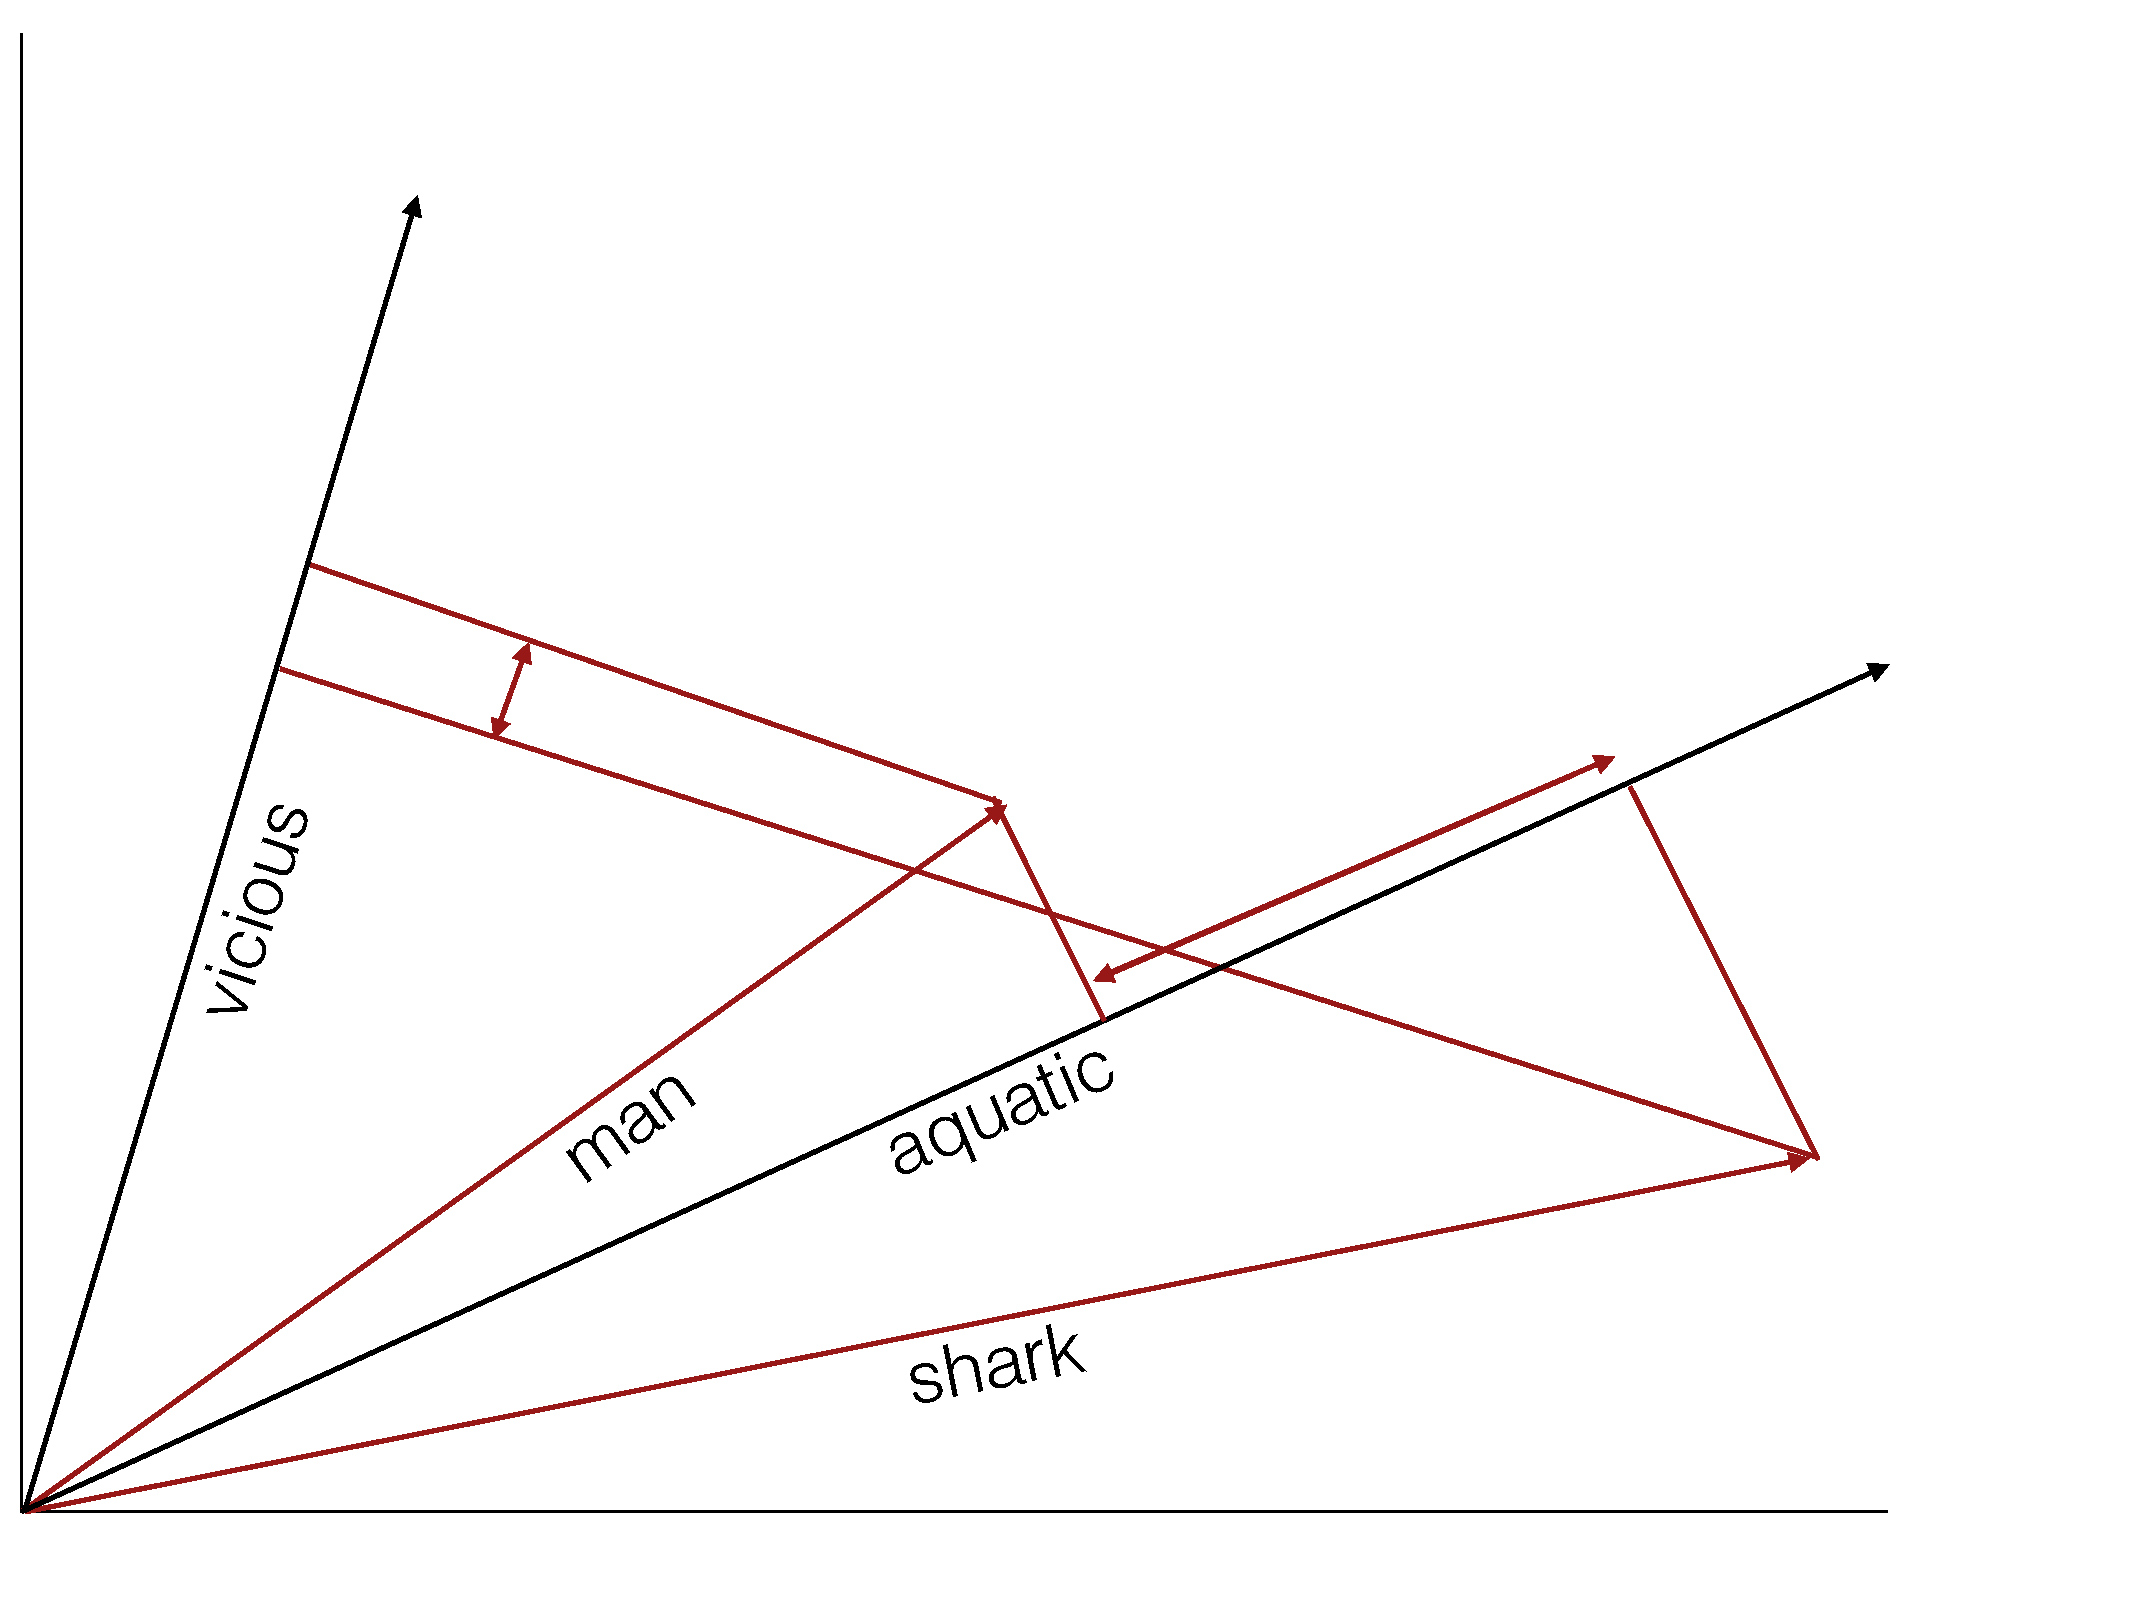
\includegraphics[height=6.5cm]{diagram2.pdf}

In this example, the vectors for \emph{vicious} and \emph{aquatic} each parametrize a QUD mapping all the points in the space (such as \emph{man} and \emph{shark}) to new points. These new points can be thought of as the positions of \emph{man}, \emph{shark} and so on in a new space which cares only about the position of the points with respect to the \emph{vicious} vector. 

Again, it is worth noting the similarly of the simple and distributional notions of QUD. In both cases, the QUD discards information, via a many-to-one mapping from worlds to sets of worlds\footnote{This is true in the distributional case because the projection  maps more than one point to a single point. Thus, we can recast the projection as a function P from a point v to the inverse image of P(v).}.

% \begin{figure}[htbp]
% \hspace*{-2.5cm}                                                           
   
%   \caption{Projection}
%   \label{fig:proj}
% \end{figure}


The intuition behind the projection is that it picks out only certain features of the original vector. For instance, we could imagine a 1 dimensional subspace which measures how \emph{predatory} an object is. This projection, if it exists, would map objects which are similarly predatory to nearby points in the space, and vice versa for points which differ in predatoriness. A higher dimensional hyperplane would care about n features, where n is the dimensionality of the hyperplane. The idea of using a projection to a hyperplane for the QUD rather than simply a projection to a line is that a metaphor might convey multiple things at once. In saying that John is a shark, we are conveying both his speed and predatory nature, but not his scaliness.

So far we have defined our QUDs in terms of projections parametrized by hyperplanes in the word vector space, but have said nothing about how these hyperplanes are to be obtained. We find that words themselves can supply the projection hyperplanes, so that we can, for instance, map the Glove vectors into the subspace parametrized by the vector (a 1 dimensional hyperplane) corresponding to the word \emph{predatory}. Thus, the $L_1$'s set of QUDs can be chosen as the projections corresponding to a set of words, such as the set of animal features in (\cite{kao}). This means that we can think of our QUDs as words, such as adjectives, which measure aspects of the subject being predicated. We can generalize to projections onto n-dimensional hyperplanes by using n-tuples of words, instead of single words.

The assumption that appropriate projections exist is based on the much observed linear substructure of word embeddings, which amounts to the claim that word vectors can be roughly decomposed as a sum of a set of other word vectors. While this linearity is very noisy, we find that it suffices for our purposes (largely, we suspect, as a result of the joint inference performed at $L_1$).

To illustrate how this works informally (but for a formal account, see section (\ref{technicaloverview})), we walk through a 2D example of our model, applied to the metaphor ``The lawyer is a shark.''. As with RSA generally, our model requires a set of possible utterances. In the present case, let us supply the possible utterances as \emph{shark} and \emph{fish}. Informally, we can describe the $L_1$ calculation of a single metaphorical expression, say ``The lawyer is a shark.'' in distributional RSA as follows:

The $L_1$ world prior over worlds w is a Gaussian with mean at $\overrightarrow{\text{lawyer}}$. The prior over QUDs q, is (in the most simple model, but see section (\ref{technicaloverview}) for variations) a uniform distribution over a set of vectors, corresponding to a set of words. Here, the QUDs might be $\overrightarrow{\text{predatory}}$ and $\overrightarrow{\text{scaly}}$.

$L_1$ then performs joint inference over worlds and QUDs, to obtain a posterior on both, following the observation of the $S_1$ utterance given w and q.

The $S_1$, in turn, takes in a world state w (a vector in the space) and a QUD (a hyperplane in the space), and has a uniform prior\footnote{We later consider weighting this prior: see section (\ref{implementation}).} over a set of possible utterances. Here, let us assume that the possible utterances are \emph{shark}, \emph{fish} and \emph{human}. The $S_1$ updates a uniform categorical distribution over the possible utterances to favor those which convey the $S_1$ world state to the listener.

% To obtain the posterior, the $S_1$ samples from $L_0$(w$'\vert$u), according to their prior P(u), and maximizes the Euclidean distance of their world state w to w$'$, after applying the projection parametrized by q to both.

The $L_0$ prior, in turn, is is identical to the $L_1$ world prior. To obtain the posterior, the $L_0$ makes the observation that $\overrightarrow{\text{shark}}$, which is the utterance they hear, is drawn from their prior distribution, and updates their prior according to this observation. The following diagram illustrates this for a 2D case, where the axes correspond to words - in practice, we use a word embedding space of 300 dimensions in which the axes have no special meaning.


% a ball representing the l0 prior, and the observed point, and an arrow for the movement


% \begin{figure}[htbp]
% \hspace*{-2.5cm}                                                           
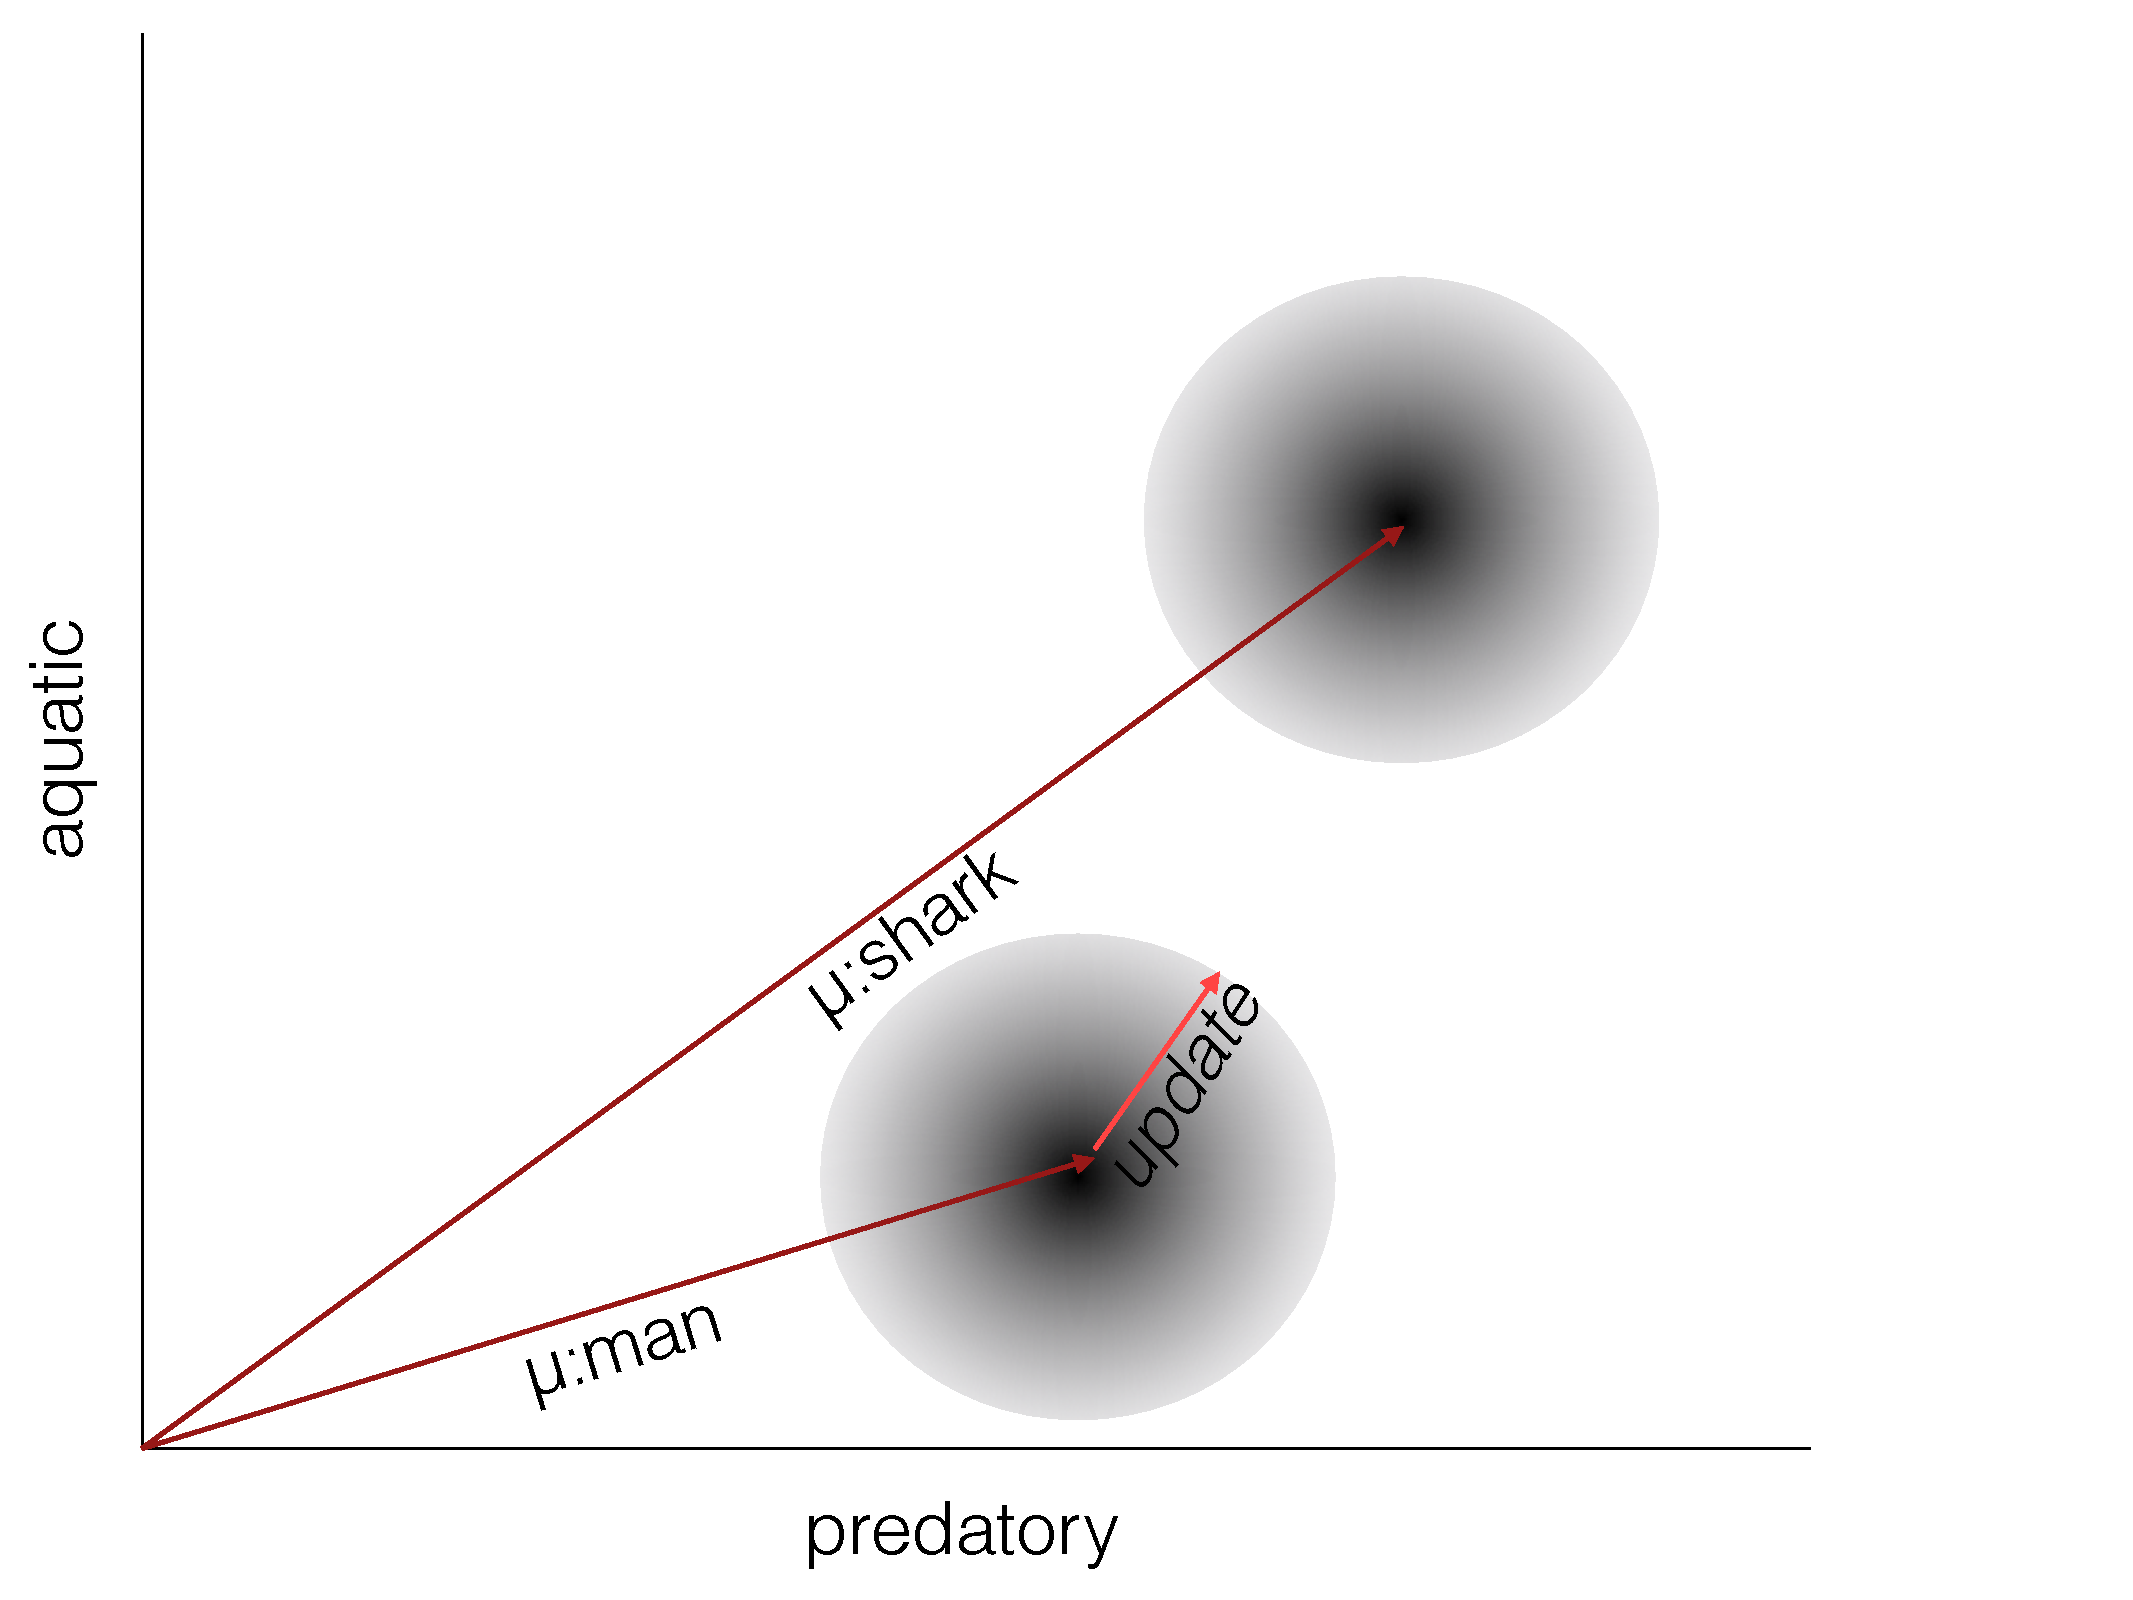
\includegraphics[height=6.5cm]{diagram1.pdf}
   
%   \caption{2D Visualization of $L_0$}
%   \label{fig:2d}
% \end{figure}




% The $L_1$ world prior, as with standard RSA, is identical to the $L_0$ world prior.

 % should place more weight on $\overrightarrow{\text{predator}}$ as a QUD than $\overrightarrow{\text{scaly}}$, and should move their world state more towards characteristics of predators than of swimmers.


Another way of thinking of DistRSA is as a spatial reference game (e.g. \cite{golland2010game}), played in a word vector space. In this setting, the $S_1$ has knowledge of what lawyers (or a particular lawyer) is like, represented by a position of the lawyer in the vector space. They also have a QUD that they care about. They choose the noun which best conveys the known position of \emph{lawyer} with respect to the QUD in question.


		% we condition on the likelihood of the $S_1$ world state being drawn from the $L_0$ posterior after having heard any given possible utterance.







\section{Technical Overview} \label{technicaloverview}

While the general format of our model is analogous to previous models in the RSA paradigm, the vectorial setting produces a number of challenges which require novel solutions.

Moreover, previous implementations of RSA have employed prior distributions for both the speaker and listener with finite support. As a result, it is possible in standard RSA to perform exact inference for the $L_0$, $S_1$ and $L_1$. By contrast, our prior is a Gaussian and as such cannot be computed via exact inference, due to the need to calculate a normalizing term which sums (or rather integrates) over an infinite set. 
% Furthermore, nesting causes approximate inference in the form of Markov Chain Monte Carlo to be unstable (see \cite{rainforth2016pitfalls}).


We therefore compute the $L_0$ and $S_1$ posteriors analytically, and use perform appromixate inference only at the $L_1$ level. We now describe how each of $L_0$, $S_1$ and $L_1$ is computed.

\subsection{Model Definition}

\subsubsection{L\textsubscript{0} Definition}

To calculate $L_0$ analytically, we make use of Gaussian conjugacy. Our $L_0$ posterior density function is defined as follows, where \emph{subject} is the word being predicated (e.g. ``lawyer'' in ``the lawyer is a shark''):

\begin{exe}
\ex $L_0(w\vert u) \propto P_{\mathcal{N}}(w\vert\mu=subject,\sigma=\sigma_1)P_{\mathcal{N}}(w\vert\mu=u,\sigma=\sigma_2)$ \label{term}
% e^f$ * e$^\mu$ \label{term}
\end{exe}
The left hand term represents the prior on the world state, and the right hand term represents the observation. By the self conjugacy of Gaussians, (\ref{term}) can be reduced analytically to a single Gaussian.

Note that truth is not a fundamental concept in distributional RSA; we have no way of saying whether an utterance is true or false. Instead, the semantics is dynamic, so that the literal meaning of an utterance is its effect on the $L_0$ prior. More precisely, the meaning of ``A is a B'' is the function from the $L_0$ prior on A to the $L_0$ posterior on A after observing B. While this deviates from traditional truth-conditional semantics, it preserves the intuition that meanings should be things which allow linguistic agents to update their world knowledge. 

The variance of the prior and observation Gaussians, $\sigma_1$ and $\sigma_2$ respectively, are hyperparameters of our model. See section (\ref{implementation}) for a discussion of their optimal values.


\subsubsection{S\textsubscript{1} Definition}

The prior for $S_1$, which is over possible utterances, is finite, and therefore is straightforward to compute\footnote{As discussed in section (\ref{rsawithqud}), having a finite set of utterances is theoretically objectionable, but for the time being, a necessary modeling assumption.}. We refer to the hyperplane which parametrizes the QUD projection as $\overrightarrow{\text{q}}$, and abuse notation by having q(v) denote the vector resulting from a projection of v along q. Note that q(v) could either be represented in the dimensionality of the original space or the projection subspace. We will assume the former, so that if v $\in$ {\rm I\!R}$^n$, q(v) $\in$ {\rm I\!R}$^n$. Then our $S_1$ is almost identical to the plain QUD RSA model:

\begin{exe}
\ex U(u,w,q) = $\log(\int_{w'} \delta_{q(w)=q(w')} * L_0(w'\vert u))$
\ex S$_1(u\vert w,q) \propto e^{U(u,w,q)}$
\end{exe}


% The utility U(u$\vert\overrightarrow{\text{q}},\overrightarrow{\text{w}}$) = $\llbracket w - L_0(w'\vert u)  \rrbracket^2$ where $\llbracket \overrightarrow{\text{v}} \rrbracket^2$ represents the Euclidean norm. We can define $S_1$ in terms of this utility function as follows:

% $S_1$(u$\vert\overrightarrow{\text{q}},\overrightarrow{\text{w}}$) $\propto$ e$^{U(u\vert\overrightarrow{\text{q}},\overrightarrow{\text{w}})}$
% q($L_0$(w$\vert$u)) * q(P(u))

\subsubsection{L\textsubscript{1} Definition}

$L_1$ is defined as follows, where P$_{QUD}$ represents the prior on QUDs. As discussed below, we can either have this be a continuous distribution over hyperplanes corresponding to projection functions, or a discrete distribution of hyperplanes corresponding to a set of n-tuples of words. In either case, we assume it is a uniform distribution:
\begin{exe}
\ex $L_1(w,q\vert u) \propto S_1(u\vert w,q) P_{\mathcal{N}}(w\vert\mu=subject,\sigma=\sigma_1)*P_{QUD}(q)$
\end{exe}
While we were able to use analytic methods to derive the $L_0$ and $S_1$ posteriors, we cannot do so for the $L_1$. Instead, we must use an approximate inference method. We try two different inference algorithms, Hamiltonian Monte Carlo (\cite{neal2011mcmc}), a brand of Markov Chain Monte Carlo inference algorithm which makes use of gradient information to move from one sample to the next, and Variational Mean Field inference (see \cite{blei2017variational}), an optimization based inference algorithm. In our first experiment we use the former, while we make use of the latter in our second, on account of its speed.

Variational Inference (VI) greatly increases efficiency over other inference methods, at the cost of requiring gradients for the $S_1$ and the functions the $S_1$ calls. Fortunately, it is possible for us to calculate these gradients, using automatic differentiation.

$L_1$ performs joint inference over QUDs and worlds. While the nature of the prior over worlds has already been discussed, two variants of $L_1$ are possible, as regards to prior on QUDs. The first is to have a categorical distribution over a set of projection hyperplanes (QUDs), for example those corresponding to n-tuples of words, according to the pretrained embedding. The output of our inference then gives us a categorical distribution over QUDs, corresponding to words (as well as a continuous distribution over worlds). 

The second variant is to have the QUD be a continuous variable. As a result of the way the projection is defined, only the angle and not the magnitude of the projection hyperplane matters. As such, we can have a uniform prior over unit hyperplanes. We will refer to these as two models as the Categorical and Non-Categorical $L_1$, respectively.

The advantage of the Categorical $L_1$ is that we can choose a particular set of QUDs, for instance, the vectors corresponding to a given set of words, and weight this prior according to the frequency of these words. This allows us to supply our model with a set of possible QUDs, and have it return a categorical distribution over them, as the $L_1$ QUD posterior.

The Non-Categorical model, on the other hand, has the contrasting benefit that no set of possible QUDs need be provided to the model. Furthermore, the use of Hamiltonian dynamics for performing the joint inference results in much faster performance. However, the Non-Categorical model yields significantly less stable results, and as such, we use only the Categorical model in our experimentation.




\subsection{Implementation} \label{implementation}

In section (\ref{rsa}) we raised the issue of scalability of RSA, relating to the need for the provision of a hand-crafted semantics, and sets of possible utterances and possible QUDs. In distributional QUD RSA, we avoid the need for a hand-crafted semantics, by using a semantics build on word vectors.

However, we attempt to go further, by also removing the need for hand chosen utterances and QUDs. This can be partly accomplished by the use of large sets of possible utterances and QUDs. We further use a language model\footnote{Introduced in (\cite{jozefowicz2016exploring}) and available at \url{https://github.com/tensorflow/models/tree/master/lm_1b}} in order to choose possible utterances in a systematic fashion.

We do this by first taking a large set of nouns from WordNet (\cite{miller1995wordnet}) and ranking them according to their probabilities of being completions of ``[subject] is a'' under the language model. We then take the first n nouns (with n varying depending on the experiment in question). So, for instance, to model ``The lawyer is a shark.'', we let the possible utterances be the best n completions of ``The lawyer is a''. The correct n varies depending on the precise task at hand - we discuss individual cases separately below. 

As for the QUDs in the Categorical model, we take a set of adjectives from WordNet, and rank them according to their cosine distance from the mean of the subject (e.g. \emph{lawyer}) and predicate (e.g. \emph{shark}). This provides a rudimentary, but useful ranking of which words are the most relevant topics for the metaphor in question. We can then generate projections from these adjectives. If we want QUD projections into multidimensional hyperplanes, we can take the cross product of our set of adjectives with itself to generate n-tuples, and then obtain the QUD projections from these.

We create categorical distributions over possible utterances and QUDs by weighting the elements in these sets according to their frequency\footnote{For a measure of frequency, we use the Google N-grams unigrams.}. Our model is computationally efficient enough that quite large inferences are possible - we can supply several thousand possible utterances and QUDs, with a run time of around 30 minutes per metaphor. 


We implemented our model in both WebPPL and Python\footnote{The code of our Python implementation will be made publicly available.}. For the later, we make use of Tensorflow, and Edward in particular (see \cite{edward}), in order to perform HMC or VI. Though the model in principle runs in both languages, the Tensorflow implementation is significantly faster, allowing us to run large inferences, over thousands of possible utterances and QUDs. Furthermore, Tensorflow and Edward are GPU compatible, allowing for significant speed up of the inference.

For our word vectors, we experimented with a number of different variants of the Glove vectors, all available at \url{https://nlp.stanford.edu/projects/glove/}. We mean center the vectors, and use PCA to remove the top 4 orthonomal bases\footnote{Rather than the bottom dimensions, as is usual for PCA. We keep the vectors in the full 50 dimensional space, rather than expressing them by their basis in the subspace.}. This second preprocessing step is inspired by (\cite{mu2016geometry}), which suggests this for improving the quality of the Glove word embeddings in particular.

% We obtained our best results with Glove840B, $\sigma_1$ of 1, and $\sigma_2$ of 0.01. We set the step size of our HMC to 0.01.



\section{Evaluation}

Our DistRSA model is evaluable in a variety of ways corresponding to various tasks. In order to test it rigorously, we run evaluations based on human judgments, both from corpora and our own experimental data. We compare our results to simpler baseline models which make use of distributional semantics but not RSA.

\subsection{Task 1: QUD Identification} \label{task1id}


The first task we attempt is metaphor understanding: the task of finding a set of words which describe suitable QUDs for a given metaphor. Before considering quantitative evaluation, we show an example of the model, performing $L_1$ inference on a limited domain, the animal-based set of 34 possible utterances and 91 1D QUDs\footnote{The hyperparameters are as follows: HMC step size: 0.25. Number of HMC samples: 1000. $\sigma_1$: 0.1. $\sigma_2$: 0.1. Speaker and listener priors: uniform.}, generated by the adjectives supplied by (\cite{kao}, page 272). 

Table (\ref{tab:l1}) displays the $L_1$'s top five QUDs (the five QUDs in the support of the $L_1$ distribution over QUDs with the most probability mass) for the subject ``man'' and the predicates ``shark'', ``sheep'' and ``lion'' respectively. Table (\ref{tab:baseline}) shows the same results, but from a vectorial baseline model, in which the ranking on the QUDs is generated by cosine distance to the mean of the vectors for the subject and predicate\footnote{We experiment with other binary operators to combine the subject and predicate vectors (sum, weighted sum, product, difference) but find that mean works best overall.}. This baseline model (which serves as a null model for the usefulness of RSA in modelling metaphor distributionally) often works well, but fails in cases where the correct QUD is not similar to either the subject or predicate. 



% ``The man is a sheep.''
% $L_0$,$L_1$ prior: multidimensional Normal around $\overrightarrow{\text{man}}$.
% $S_1$ distribution over utterances : uniform over: $\overrightarrow{\text{sheep}}$, $\overrightarrow{\text{cat}}$,$\overrightarrow{\text{dog}}$...\footnote{For full set, see appendix.}
% $L_1$ distribution over QUDs:


\begin{table}[ht]
	\label{tab:l1}
	\caption{L1 model}
	\centering
	\begin{tabular}{rlll}
	man (is a) & shark & sheep & lion \\\toprule
	1. & predatory & unfree & majestic \\
	2. & unfree & dry & ferocious \\
	3. & unattractive & wild & tame \\
	4. & slimy & artless & fierce \\
	5. & sighted & dependent & loyal \\\bottomrule
	\end{tabular}
\end{table}

\begin{table}[ht]
	\label{tab:baseline}
	\caption{Baseline model}
	\centering
	\begin{tabular}{rlll}
	man (is a) & shark & sheep & lion \\\toprule
	1. & wild & wild & wild \\
	2. & dangerous & small & large \\
	3. & large & large & small \\
	4. & predatory & dangerous & blind \\
	5. & small & mean & big \\\bottomrule
	\end{tabular}
\end{table}



We suggest that the advantage that DistRSA offers over the baseline is simply the dynamics of RSA generally: the model takes into account not only the observed utterance, but possible alternatives, giving rising to an ``explaining away'' effect discussed in section (\ref{rsawithqud}). For example, the $L_1$ would be unlikely to infer that ``The man is a cat'' conveyed stubbornness, since ``The man is an ox.'' is an alternative which performs this task better.

Qualitatively, these results are promising: for the most part, the QUDs identified seem appropriate. Note that the QUD should not be taken as a paraphrase of the metaphorically used noun. For instance, \emph{tame} is a suitable QUD for ``The man is a lion.'', because tameness is a topic that the use of the metaphor resolves, even though lions are the opposite of tame. 

\subsubsection{Mechanical Turk Experiment}

\paragraph{Participants} For quantitative evaluation, we obtained human judgments from 40 Mechanical Turk participants. 


\paragraph{Materials} We collected 15 metaphors from COCA (\cite{davies2008corpus}), by searching for ``[Singular Noun] is like a [Singular Noun]'', and using hand-chosen pairs of nouns obtained from this search as our metaphor set\footnote{Collecting data from COCA has precedent in other computational work on metaphor, e.g. (\cite{neuman2013metaphor}) and (\cite{turney2011literal})}.


\paragraph{Procedure} We used Mechanical Turk to obtain crowd-sourced judgments regarding each metaphor. Each participant was shown all 15 of the metaphors (order randomized). For each metaphor, they were shown 6 adjectives, 3 from the $L_1$ and three from the baseline described above, which simply finds the words nearest to the mean of the subject and predicate (order also randomized). They were instructed to rate the relevance of each adjective to the metaphor, where relevance is defined as follows: ``an adjective is relevant if it describes a property of the subject (e.g. ``the man'' in ``The man is a shark'') that the speaker of the sentence is trying to talk about''. The format of the experiment is displayed in Figure (\ref{fig:1}). The baseline model was supplied with the same 50 QUDs to rank that constitute the $L_1$ QUD distribution support.

\begin{figure} \label{screenshot}
\centerline{\includegraphics[width=\linewidth,height=7cm]{mturk-screenshot.pdf}}
\caption{A slide from our Mechanical Turk experiment.} \label{fig:1}
% $L_1$}
 % and baseline models, per metaphor.}
\end{figure}

For the $L_1$, we took the first 50 possible utterances generated by our pretrained language model (\cite{jozefowicz2016exploring}), and for QUDs, take the pairs of words\footnote{In fact, we exclude all pairs where $w_1=w_2$.} $\langle$w_1,w_2$\rangle\in$W$\times$W, where W consists of the first fifty QUDs generated as described in section (\ref{implementation}). 

The hyperparameters of the model are as follows: VI step size = 0.0005. Sigma$_1$ = 0.0005. Sigma$_2$ = 0.005. Dimensions onto which QUD is projected: 2. Number of QUD tuples = 1225. Speaker prior: uniform. Listener prior: uniform. GloVe vectors: Twitter, 25 dimensional.

We obtain these hyperparameters by qualitative examination of the behavior of the model on a small validation set of metaphors. We find that the choice of GloVe vectors has little impact on the quality of results, but that the values of the sigma$_1$ and sigma$_2$ are important. Moreover, results seem to improve qualitatively when the QUDs project into a subspace of more than 1 dimension. 

\section{Results}

\subsection{Results for Task 1}


We ran a linear mixed effects model, predicting slider rating from baseline vs. $L_1$ metaphor, with by-metaphor and by-participant random intercepts, to analyse the results of the experiment. We find a significant correlation ($\beta$=0.32,SE=0.01027, t=9.789, $\chi^2$=94.57, p$<$0.0001) between an adjective being from our model and it being rated higher on the scale of relevance\footnote{Our p-value and $\chi^2$ are obtained by a log-likelihood ratio test.}.


\begin{figure} 
\centerline{\includegraphics[width=\linewidth,height=8cm]{barchart}}
\caption{The mean user rating for our model vs. the baseline model, per metaphor. Error bars indicate bootstrapped 95\% confidence intervals.} \label{resultsbar}
% $L_1$}
 % and baseline models, per metaphor.}
\end{figure}

As can be seen in Figure (\ref{resultsbar}), there is a lot of variation in the average quality of proposed adjectives across both models, between metaphors. For the baseline model, we note that there is a subset of metaphors for which the baseline will perform well, as discussed in section (\ref{task1id}). These are metaphors where good QUDs q are such that the subject and predicate are close when projected along q. In these cases, averaging the subject and predicate will generally give rise to a good QUD. 

However, further work is necessary to understand the conditions under which our model fails, and what could be done to improve it. An example of a failure case is the ranking of ``adoptive'' as the best QUD for the metaphor ``The father is a shark.'' - in this case, it is not clear why the model chose this particular adjective. A further challenge, therefore, is to develop methods to interpret the choices made by the model, so that the model's posterior distributions can be understood in terms of the underlying geometry of the word embedding space.



% We use a mixed effects model to control for variation between participants. Our findings are as follows: participants prefer our model with 514 out of 980 of the total binary choices for our model. On a binomial test, this yields a p-value of 0.13. 


% For our quantitative testing of the QUD identification system, we consider three domains: the animal metaphors described above, a set of verbal metaphors, and a set of adjective-noun phrases collected by (\cite{tsvetkov2014metaphor}). We use the model described in the second of the above examples.

% For each, we first crowd-source good and bad QUDs for the metaphors in question. For instance, in the animal domain, we ask participants to provide 2 relevant attributes, i.e. adjectives describing sharks that are communicated about men in ``The man is a shark.'' and 2 irrelevant attributes. We see this as a way of obtaining QUDs. For each metaphor, we then use our model to produce predictions, and find the rank of the two pairs of adjectives in a 2-dimensional inference. We judge the model to have performed correctly if it ranks the pair of relevant adjectives above the irrelevant ones. 

% We secondly ask participants to judge the top 3 QUDs supplied by the DistRSA model against those generated by the null model described above. We judge the model to have performed correctly if the participant prefers the choices of the real model.


% In order to show that domain-specific knowledge need not be input to the model, we perform our evaluations on the \emph{non-categorical} $L_1$, with a fixed set of the top 1000 most common nouns as possible utterances.


% Metaphor understanding constitutes the inference of the QUD from a metaphorical utterance, on the part of a listener. Metaphoric composition constitutes the inference of a posterior world state from a metaphorical utterance, on the part of a listener.
\subsection{Task 2: Metaphor Detection} \label{task2det}

A second task to which our model can be applied is metaphor detection. We model the process of metaphor detection as an inference as to the existence of a QUD projection at all. For a given expression, if the QUD inferred by the $L_1$ to have the most weight is the trivial projection (the identity function), then we conclude that the expression is literal. Otherwise, we conclude that the expression is metaphorical. For instance, this system should identify ``The lawyer is a shark.'' as metaphorical and ``The lawyer is a judge.'' as literal.

For this task, we use the labeled corpus of data provided by (\cite{tsvetkov2014metaphor}). This consists of 884 metaphorical, and 884 non-metaphorical, adjective-noun phrases, collected by two annotators from text corpora. For instance, an example of a literal AN phrase is ``hollow tree'', while an example of a metaphorical one is ``hollow victory''.

We use 84 of each of the two lists of AN phrases as a training set for our system, for fitting hyperparameters of our categorical model. We test on the remaining 711 of each, having removed 89 metaphors in each to exclude words which did not appear in GloVe\footnote{The hyperparameters are as follows: HMC step size = 0.0005. Number of HMC samples = 400. Burn in: 285 removed. Sigma$_1$ = 0.0005. Sigma$_2$ = 0.01. Number of possible utterances = 30. Dimensions onto which QUD is projected (if not trivial QUD): 1. Number of QUD 1-tuples (including trivial QUD) = 31. Speaker prior: uniform. Listener prior: 0.9 on trivial QUD, 0.1 uniformly distributed between other 30 QUDs. GloVe vectors: twitter, 25 dimensional, with mean centering of vectors and removal of PCA top dimensions.}.

\subsection{Results for Task 2}

The results of this experiment are as follows. For each item in the test set, we see whether the trivial QUD has the most weight out of the set of QUDs. If it does, we say that the system has classified the AN phrase as being literal. The expectation is that the system should more commonly classify the phrases in the metaphorical AN set as metaphors and those in the literal AN set as literal.

This is indeed the case, with 356 out of 711 metaphorical AN phrases classified as literal, compared to 439 out of 711 literal AN phrases classified as literal. This yields p$<$0.0001 (with the null hypothesis that this result is drawn from a binomial distribution with equal likelihood of either outcome.). 

% Another way of measuring the importance of the trivial QUD is by its probability density divided by the cosine distance between the adjective and noun in question. This division addresses a confound caused by the effect that the distance between these words has on increasing the trivial QUD density. In this case, the sum of all trivial QUD densities divided by cosine distance of the adjective and noun, across the 711 metaphorical AN phrases, is  303.3. For the literal AN phrases, it is 498.3.

This experiment suggests that the density of the trivial QUD is indeed an indicator of the literalness of a metaphor. A preliminary theoretical conclusion we might draw is as follows: while metaphorical and literal expressions lie on a continuum, the usefulness of QUDs is higher for metaphorical expressions.

While it is possible to fit a classifier to the data, by classifying those AN phrases as metaphors which yield a trivial QUD density below some fit threshold (e.g. 0.05), this results in accuracy of around 0.55, which is considerably less than comparable baselines (\cite{tsvetkov2014metaphor}), which yields an accuracy of 0.86. As such, without further tuning, the system proposed here is not yet suitable for state of the art metaphor detection.


% [NB: this is currently still being tuned: results look to be about at 70\% accuracy at the moment. Aim is to tune to 80\%]


% \begin{table}[ht]
% 	\label{tab:baz}
% 	\caption{Some data}
% 	\centering
% 	\begin{tabular}{rlll}
% 	 & Gold Label: T & Gold Label: F \\\toprule
% 	Prediction: T & \% & \% \\
% 	Prediction: F & \% & \% \\\bottomrule
% 	\end{tabular}
% \end{table}

% \subsection{Task 3: Metaphor Generation}

% A third task is metaphor generation: this is a system which generates novel metaphors given a world state and QUD: from the perspective of RSA, it is the output of a metaphorical speaker model. The sensible choice of speaker is S$_2$, since the $S_1$ does not reason about a pragmatic listener. 

% We consider two variants of the S2

% 	explain the s2 etc

% 	for the time being, we merely present qualitative results for this system

% \subsection{Task 4: Paraphrase}
%
% Finally, we can consider the task of metaphor paraphrase, where a metaphorical word is replaced with a more ``literal'' paraphrase in a given context. For instance, given ``The lawyer is a shark.'', the paraphrase system should produce something like ``The lawyer is ruthless and merciless.''.


% \section{Discussion} \label{discussion}



% 		that both metaphorical adjectival modification and predication can be treated with the same mechanism



% In this paper, we have considered two sorts of metaphor: copular predication and adjectival modification. In logical semantics, copular predication takes a noun and forms a sentence, while adjectival modification takes a noun and returns a noun phrase. 
	

% Despite this difference, we have proposed that the same mechanism, namely our metaphor model, can handle both.
	

	% while these have different types in logical semantics (in logical semantics, copular predication ($\lambda$x. x is a B) takes a noun and forms a sentence - it is of type (e$\to$t). Adjectival modification ($\lambda$x. y x) takes a noun and returns a noun phrase - it is of type (e$\to$t)$\to$(e$\to$t) )


	% .With these two instances of composition in mind, we can consider the theoretical question of the distinction between literal and metaphorical meaning.

\section{Discussion}
\subsection{The Extent of Metaphor} \label{litvsmet}

\emph{Prima facie}, it seems that some predications and modifications are metaphorical, while others are literal. As far as our model is concerned, metaphorical meaning is distinguished from literal meaning by requiring a QUD to be interpreted. 


% \footnote{It is important to note that the literal-metaphorical distinction is separate from the semantics-pragmatics distinction. In our model, the former concerns the use of QUDs, while the latter concerns whether the listener is $L_0$ or $L_n$ for n$>$0.}.

A natural question which arises, therefore, is as to the extent of metaphorical language. For instance, many AN phrases normally treated as ``literal'' could be understood to require a QUD for interpretation. This line of argument is proposed by philosophers such as Quine:
	\begin{quote}
		``Quine pointed out that a red apple is red on the outside while a pink grapefruit is pink on the inside, and Partee took that example to be similar to the case of ``flat'' which applies differently in ``flat tire'',``flat beer'' and ``flat note''...''. - (\cite{lahav}) 
	\end{quote}


The point here is that even the most seemingly literal modifier, the color term \emph{red}, in fact has different meanings depending on the noun to which it is applied. In our terms, the QUD for ``flat tire'' is a projection which cares about \emph{deflation}, while for ``flat beer'', it is a \emph{fizziness} projection. Similarly for predicative metaphor, ``The grapefruit is pink.'', like the AN phrase ``the pink grapefruit'' requires us to discern which aspect of the grapefruit is pink. Generalizing this line of thinking, we could entertain the following hypothesis:

% For instance, ``John is a musician.'' might either mean that John is musically talented, or that he plays music for a career. In other words, the aspect in which John is a musician is underspecified, and needs to be inferred.

\begin{exe}
\ex All modification and predication requires the inference of QUDs for interpretation (and by our definition, is metaphorical) \label{prop3}
\end{exe}

The claim in (\ref{prop3}) is that all modification and predication in natural language must be interpreted at the QUD RSA $L_1$, not at the $L_0$. It is important to make clear that this claim does not entail that there is no such thing as semantics, separate from pragmatics; in fact, our RSA model makes a very clear distinction between the two. 

For DistRSA, the semantic meaning of each lexical item is a vector. The mapping from lexical items to vectors, for which we use GloVe, parametrizes the model's semantics. GloVe itself encodes pragmatic information; for instance, the co-occurrence of \emph{shark} and \emph{man} arising from instances of the metaphor ``The man is a shark.'' in GloVe's training data, influences the position of the vectors for \emph{shark} and \emph{man}. However, this mapping from words to vectors need not, in principle, be influenced by pragmatics. For example, (\cite{monroe2015learning}) is an RSA system which learns a semantics while making pragmatic observations, allowing the semantics to be separate. We hypothesize that a similar technique could in used in the context of DistRSA, allowing for a mapping from words to vectors which only captures information that the RSA would not account for itself. 



\paragraph{Intersectivity and Metaphor} 

Closely related to the issue of (\ref{prop3}) is the status of \emph{non-intersective} adjectives. Intersective adjectives are those which obey the following property: for an intersective adjective A, if A$_x$ is the set of things which are A, and for a noun N, if N$_x$ is the set of things in the extension of that noun, then the intersection of these two sets is the extension of [A N]. For example, if one believes that \emph{red} is an intersective adjective, then the set of red apples would be the intersection of the set of red things and the set of apples.

As seen by Quine's position on ``red'' and ``pink'', there are grounds for skepticism that color terms are really intersective. Along the lines of (\ref{prop3}), we might instead arrive at the position that all adjectives are non-intersective, being instances of metaphorical modification.
% We see this as roughly comparable to the theoretical position of (\cite{roberts1996information}), who envisions that all utterances in natural language are interpreted with respect to a question under discussion. 

The results from the metaphor detection experiment shed some light on these issues. AN phrases, as seen in the metaphor detection experiment, get assigned differing weights for the trivial QUD projection in the $L_1$ inference. One way of interpreting the weight assigned to this QUD is as the degree of literalness of the phrase or sentence in question. On this approach, metaphorical and literal meaning are part of a continuum; the more metaphorical an utterance is, the more the QUDs matter for its interpretation. From this perspective, (\ref{prop3}) would amount to the claim that no AN phrase is fully literal.

The issue is further complicated by a diachronic dimension; predication which once would have required pragmatic inference of a QUD no longer does. For instance, to understand ``John is a fool.'', it is highly unlikely that a listener will be unaware of the conventionalized meaning of ``fool'' as someone stupid and have to infer it. Thus, it does not seem to be the case that metaphorical pragmatic inference is required to understand what is conveyed by ``John is a fool'', ``Jane is a cougar.'' or ``Time flies.''.  


% However, as discussed in section (\ref{litvsmet}), even color adjectives seem not to behave intersectively, on detailed examination. 
% From a distributional perspective, this intuition is bolstered by the findings of (\cite{boleda}), which fails to distinguish intersective (or in their terms, extensional) and non-intersective (or intensional) adjectives on distributional grounds.



% \begin{exe}
% \ex Non-intersective adjectives are adjectives that are used metaphorically. \label{prop2}
% \end{exe}



%  If \emph{gray} is not intersective, then 



% The contribution of \emph{non-intersective} adjectives depends on the noun they modify. For instance, a good dancer is good in a different way to a good cook\footnote{Note that \emph{good} is also a relative scalar adjective (c.f. \cite{kennedy}). This is an orthogonal property, however.}. 

% There is a clear parallel to metaphorical adjective use here; non-intersective adjectives modify different nouns differently, as a result of focusing on different attributes. A good juggler is good with respect to the juggler's skill, while a good meal is good with respect to the meal's taste. Non-intersective adjectives are typically considered separate from adjectives used metaphorically, but it is not obvious that this should be the case. An alternate hypothesis is as follows:

% In fact, as an extension of (\ref{prop1}), we could consider the following hypothesis:



% While our model was designed to the end of modeling metaphor computationally, it raises a number of theoretical questions. Firstly, we apply our model to both metaphorical predication (section \ref{task1id}) and metaphorical modification (section \ref{task2det}). 



% . If we explain intensionality as metaphorical language use, then the ubiquity of intensional adjectives is simply an instance of the more general claim that above

% The idea that adjectival modification in general should be modeled in the manner of metaphorical modification can be extended to predicative metaphor of the form ``A is a B''. 



% To test (\ref{claim}) empirically, we can ask whether apparently literal copular predicates and AN phrases can be treated in our model in the same way as metaphorical ones.


% The claim (\ref{prop2}), in conjunction with (\ref{prop3}), raises another possibility, namely (\ref{prop4}):

% \begin{exe}
% \ex There are no intersective adjectives. \label{prop4}
% \end{exe}

% This is to propose that all apparently intersective adjectives are really non-intersective, and ought to be interpreted with QUDs.




\subsection{Compositional Distributional Semantics}

Logical semantics for natural language captures compositionality well, but falls short on certain aspects of word meaning, particularly in representing the similarity or difference between words. Distributional models of NL semantics address this by offering useful similarity metrics. As such, an active topic of research (\cite{socher2013recursive}, \cite{coecke2010mathematical}) is \emph{compositional distributional semantics}. The key challenge of this research is to calculate meanings (vectors) for phrases and sentences, in terms of the meanings for words.

Our model sheds some light on this problem when $L_1$ inference is recast as a method of noun-adjective composition. The idea is this: a noun phrase like ``fiery temper'' should exist in the same space as ``temper'', since they are of the same type\footnote{The analogy between types and vector spaces is explored formally by \cite{coecke2010mathematical}, which proposes a mode of composition for distributional semantics which shares properties of standard semantic composition.}. We can therefore make the following claim:
\begin{exe}
\ex If the meaning of [NOUN] is the prior of $L_1$, then the meaning of [ADJECTIVE NOUN] is the posterior of $L_1$ after hearing [ADJECTIVE]. \label{prop1}
\end{exe}

In other words, the move from $L_1$ prior to posterior (the process of inference) can be understood as the function by which an adjective modifies a noun.

If this hypothesis is true, it should be possible to calculate vectors for compositional units such as AN phrases using our model, provided that the adjective in question is used metaphorically (but see section (\ref{litvsmet}) for a discussion of the extent to which most or all adjectival modification is metaphorical). This is beyond the scope of the present work.

These proposals, (\ref{prop3}) and (\ref{prop1}), clearly need more empirical research before even initial conclusions can be reached. We simply raise the discussion as a reminder that distributional models such as the one proposed here may apply to predication and modification generally, rather than the rather narrow cases for which it first seems appropriate.



% By contrast, many semantic models propose that there exists a set of intersective adjectives. 

% We can test this hypothesis by investigating whether our system for metaphor is capable of modeling the behavior of intensional adjectives.

% [Left empty until I decide whether to include this section]

% This question has a long history in the philosophy of language. 
% 	One camp (c.f. \cite{cappelen2004tall}) argues for a fixed literal meaning, on top of which while the other is skeptical of this notion entirely (c.f. \cite{recanati}), and argues that inasmuch as meaning is either, it is all metaphorical.

% \subsection{Intersectivity and Metaphor}

% A related line of inquiry to the metaphor-literal meaning continuum regards intersective and subsective adjectives. These are adjectives which do or don't observe the following property, respectively:

% 		\begin{exe}
% 		\ex $\llbracket ADJ NOUN \rrbracket = \llbracket ADJ \rrbracket \cap \llbracket NOUN \rrbracket$
% 		\end{exe}

% Here, the question arises of which adjectives are truly intersective, and whether apparently intersective adjectives are really subsective. (\cite{boleda}), for instance, studies the distributional properties of intersective and subsective adjectives, and is unable to find a difference in the way they modify nouns.


% This reduces to the debate over the extent of metaphor if we entertain the following possibility:
% 		\begin{exe}
% 		\ex Hypothesis: subsective adjectives are just adjectives which are interpreted metaphorically.
% 		\end{exe}



% \subsection{Compositional Distributional Semantics}

% While distributional semantics has proved invaluable to computational linguistics in recent years, it operates largely on a lexical level. As such, the correct method of composing word vectors into phrase and sentence vectors is an open question. 

% We offer the possibility that QUD RSA is a means to achieve composition

% \subsection{Conventionalization}

% We set out by noting the semantic productivity of metaphor. However, it is clear that common metaphors are conventionalized to some degree. For instance, to say that a person is a sheep is a common idiom, and as such

% However, 

% ``The fact that nearly all uses of metaphorical collocations
	% are at least partially conventionalized should not obscure
	% the fact that metaphorical language in general can be
	% productive. ''

% From our perspective, metaphorical meaning is meaning which requires a QUD to interpret. Therefore, in the context of our model of metaphorical predication, we can instantiate this to a more specific question: are there utterances of the form ``A is a B'' for which the correct QUD is the trivial one (i.e. the identity projection)? Such utterances would correspond to genuine literal statements. For instance, it might be argued that in ``That fish is a shark.'', all aspects of sharks are relevant for the predication.

% Empirical evidence can be brought to bear on this debate. Recalling the proposed link between intensional adjectives and metaphor, 
%
%
%
% 	Lahav dismisses Partee's examples as cases of ``mere metaphor''.



\section{Conclusions}

On the one hand, we have developed a model of metaphor which performs well on a range of tasks. On the other, we have extended RSA to a distributional semantics, showing that the Bayesian approach to pragmatics can scale successfully to multidimensional continuous distributions. This scaling not only absolves the need for a hand-built semantics, but also for a hand-specified set of possible utterances and QUDs, since we can supply these both in a procedural way.

Of course, there are many ways in which the language which DistRSA models is not natural. For instance, we only treat very simple cases of metaphor, and model them in a way which ignores context, as well as the effect of words other than the subject and predicate. Furthermore, the speaker in our model has a finite set of possible utterances as a prior. This runs against basic theoretical insights regarding the productivity of language.

To address these shortcomings, a natural extension to our model would be the use of a neural speaker and listener (a direction pursued for simpler RSA models by \cite{andreas} and \cite{monroe2015learning}). Not only would this allow DistRSA to intake unprocessed language from an NL corpus, it would also result in a speaker who could produce potentially infinite utterances.

\printbibliography

\end{document}